\chapter{Tinjauan Pustaka dan Dasar Teori}

\section{Tinjauan Pustaka}
\subsection{\textit{Chatbot} dengan Sistem Berbasis Aturan (\textit{Rule-Based System})}
Sistem berbasis aturan (\textit{rule-based system}) merupakan salah satu pendekatan yang paling awal dalam pengembangan \textit{chatbot}.
Dalam sistem ini, alur percakapan, pertanyaan yang dapat dikenali, serta respons yang diberikan telah ditentukan sebelumnya melalui serangkaian aturan eksplisit.
Aturan-aturan tersebut umumnya dirancang secara manual oleh ahli di bidang tertentu.
Sebagai contoh, dalam konteks kesehatan mental, perancang aturan bisa berupa psikiater, psikolog, atau peneliti di bidang kesehatan.
Implementasi dari aturan-aturan tersebut dapat berbentuk struktur kondisional seperti \textit{if-then-else} yang digunakan untuk mengatur jalannya percakapan.
Karena aturan-aturan ini tertulis secara eksplisit, pengembang memiliki kendali penuh terhadap arah percakapan dan jawaban yang diberikan oleh \textit{chatbot}.
Hal ini memungkinkan \textit{chatbot} merespons pertanyaan pengguna secara konsisten dan sesuai dengan skenario yang telah ditentukan.

Salah satu pionir \textit{chatbot} berbasis aturan adalah ELIZA, yang dikembangkan oleh Joseph Weizenbaum di Massachusetts Institute of Technology (MIT) pada tahun 1966.
ELIZA dirancang untuk menyimulasikan percakapan antara pasien dan psikoterapis aliran Rogerian, dengan memanfaatkan teknik \textit{pattern matching} (pencocokan pola) dan \textit{substitution} (penggantian kata).
Sistem ini mencocokkan masukan pengguna dengan pola-pola tertentu yang telah didefinisikan dalam skrip. Pola-pola tersebut biasanya mengandung \textit{wildcard} seperti simbol * (\textit{asterisk}), yang memungkinkan sistem menangkap frasa dari masukan pengguna dan menyusunnya kembali dalam bentuk respons yang sesuai \cite{Weizenbaum1966ELIZA}.

Di Indonesia, salah satu contoh implementasi \textit{chatbot} berbasis aturan adalah Lintang, sebuah \textit{chatbot} yang dikembangkan oleh HPU UGM.
\textit{Chatbot} ini dirancang untuk melakukan skrining awal masalah kesehatan mental dan memberikan pertolongan pertama psikologis.
Lintang dilengkapi dengan berbagai fitur utama seperti psikoedukasi yang menyediakan informasi penting mengenai kesehatan mental, termasuk berbagai gangguan, gejala, dan strategi bantuan diri.
Tips kesehatan mental yang memberikan saran untuk merawat dan meningkatkan kesehatan mental, seperti teknik relaksasi, manajemen stres, dan promosi kesejahteraan emosional.
Fitur swaperiksa yang memungkinkan pengguna melakukan evaluasi awal kondisi kesehatan mental dengan menjawab sejumlah pertanyaan.
Terakhir, direktori layanan yang menyajikan informasi mengenai sumber daya dan layanan kesehatan mental yang tersedia di lingkungan fakultas maupun universitas \cite{Lintang}.

Sistem berbasis aturan menawarkan keunggulan dari segi kontrol penuh akan alur percakapan dan respons yang dihasilkan.
Hal tersebut menjadikannya cocok diimplementasikan pada aplikasi yang membutuhkan struktur dialog ketat dan dapat diprediksi seperti pada ELIZA dan Lintang.
Namun, pendekatan ini memiliki tantangan pada skalabilitas dan fleksibilitas.
Sistem akan menjadi sangat kompleks dan sulit untuk dipelihara seiring bertambahnya variasi masukan pengguna karena semua aturan harus di bangun secara manual.
Selain itu, \textit{chatbot} cenderung tidak mampu untuk memahami dan menangani percakapan yang sifatnya terbuka atau tidak terduga.


\subsection{\textit{Chatbot} dengan \textit{Fine-Tuning Large Language Model}}
\textit{Chatbot} mengalami perkembangan yang signifikan seiring dengan kemajuan teknik \textit{Natural Language Processing} (NLP), khususnya dengan adanya \textit{Large Language Model} (LLM) seperti GPT, Gemini, Qwen, Llama, dll.
LLM memungkinkan terjadinya interaksi percakapan yang luwes antara manusia dan mesin.
\textit{Language model} ini dilatih menggunakan sumber data yang masif, sehingga mampu memahami dan menghasilkan teks dengan konteks yang luas dan alami.
Namun, LLM mengalami kesulitan saat diimplementasikan pada kasus yang spesifik, seperti menjadi \textit{chatbot} kesehatan mental untuk suatu instansi.
Jawaban yang diberikan LLM sering kali bermasalah, seperti terlalu umum, berhalusinasi, dan tidak faktual.
Untuk itu, banyak dikembangkan metode seperti \textit{fine-tuning} untuk menutupi celah tersebut.

\textit{Fine-tuning} banyak dilakukan untuk melatih suatu \textit{language model} sehingga dapat sangat mahir pada domain tertentu.
Sebuah penelitian oleh Yu pada tahun 2024 mencoba mengeksplorasi metode untuk meningkatkan performa \textit{chatbot} untuk dukungan kesehatan mental.
Penelitian tersebut menunjukkan adanya peningkatan performa umpan balik \textit{chatbot} setelah dilakukan \textit{fine-tuning}.
Hasil evaluasi menunjukkan penggunaan \textit{fine-tuning} pada LLM DialoGPT (sekitar 1,5 B parameter) memiliki kualitas percakapan yang lebih relevan dan akurat, dengan skor BLEU mencapai 0,32 yang lebih tinggi dibandingkan GPT 3 (sekitar 175 B parameter) tanpa \textit{fine-tuning} yang hanya mencapai 0,13 \cite{yu2024FineTuneOnMentalHealthChatbotExperimental}.
Dari hasil tersebut terlihat potensi besar \textit{fine-tuning} dalam meningkatkan performa LLM untuk kasus tertentu.

\textit{Fine-tuning} terbukti secara signifikan meningkatkan performa \textit{language model} dalam menghasilkan umpan balik yang lebih relevan dan kontekstual, sebuah kapabilitas yang krusial khususnya dalam aplikasi layanan kesehatan mental.
Tingkat keberhasilan peningkatan ini sangat ditentukan oleh kualitas dan relevansi data yang digunakan selama proses \textit{fine-tuning}.
Model yang dihasilkan secara inheren akan mencerminkan karakteristik data pelatihannya.
Meskipun demikian, implementasi \textit{fine-tuning} menghadapi tantangan, terutama ketika berhadapan dengan basis pengetahuan yang sering berubah atau dinamis.
Kebutuhan untuk melakukan \textit{fine-tuning} ulang secara berkala demi menjaga model tetap \textit{up-to-date} memerlukan alokasi sumber daya komputasi yang besar, baik dari segi waktu, maupun daya pemrosesan.


\subsection{Penggunaan \textit{Prompt Engineering} pada \textit{Large Language Model} (LLM)}
\textit{Large Language Model}, yang dilatih pada korpus data tekstual masif, menunjukkan kinerja yang luar biasa dalam berbagai tugas pemahaman dan \textit{text generation}, bahkan sering melampaui manusia pada tugas pengetahuan umum.
LLM beroperasi dengan mengkodekan input teks ke dalam suatu ruang vektor berdimensi tinggi yang merepresentasikan hubungan semantik antar kata dan frasa.
Representasi vektor tersebut yang kemudian menjadi dasar bagi model untuk menghasilkan output teks yang relevan, koheren, dan sesuai dengan konteks yang diminta.
Kualitas respons dapat dipengaruhi oleh berbagai faktor, termasuk \textit{prompt} yang diberikan, \textit{hyperparameter} model, dan keragaman data pelatihan \cite{Chen2025UnleashingPotentialPromptEngineering}.
Dalam aplikasinya \textit{prompt} merupakan input dari model, mengubah \textit{prompt} dapat menghasilkan hasil yang berbeda secara signifikan \cite{Kaddour2023ChallengesApplicationsLLM}.
Untuk itu, \textit{prompt engineering}, pendekatan sistematis dalam merancang \textit{prompt}, memiliki peran krusial dalam memaksimalkan kinerja LLM.


Publikasi \textit{"Language Models are Few-Shot Learners"} oleh Brown et al. 2020 memberikan gambaran bahwa LLM seperti GPT-3 dapat dimaksimalkan dalam menyelesaikan tugas NLP menggunakan metode \textit{in-context learning} \cite{LLMisFewShot2020}.
\textit{In-context learning} merupakan paradigma dalam \textit{Natural Language Understanding} (NLU), di mana demonstrasi tugas ditambahkan ke dalam input \textit{prompt} sehingga \textit{pre-trained model} dapat menangani tugas tersebut tanpa memodifikasi parameter di dalamnya \cite{Dong2024SurveyInContextLearning}.
Penelitian ini membuka pengetahuan baru bahwa untuk memaksimalkan sebuah model dalam suatu tugas khusus dapat dilakukan tanpa memodifikasi bobot model (\textit{fine-tuning}).
Model yang cukup besar dapat "belajar" untuk melakukan tugas hanya dari beberapa contoh yang diberikan dalam \textit{prompt} itu sendiri, tanpa memodifikasi model itu sendiri \cite{LLMisFewShot2020}.
Brown et al. mengeksplorasi tiga variasi \textit{in-context learning} yang dibedakan berdasarkan banyaknya contoh demonstrasi yang diberikan dalam \textit{prompt}, sebagai berikut.

\begin{enumerate}
	\item \textbf{\textit{Few-Shot Prompting}} \\
	      Model diberikan beberapa contoh demonstrasi tugas pada saat inferensi. Suatu contoh biasanya memiliki konteks dan penyelesaian yang diinginkan.
	      \textit{Few-shot} bekerja dengan memberikan $K$ buah contoh konteks dan penyelesaiannya, diikuti oleh input target yang harus diselesaikan oleh model.
	      $K$ biasanya berentang antara 10 s.d 100 bergantung dengan \textit{context window} model \cite{LLMisFewShot2020}.
	\item \textbf{\textit{One-Shot Prompting}} \\
	      Model diberikan 1 contoh demonstrasi ($K=1$) beserta deskripsi dari tugas yang akan dikerjakan dalam bahasa alami.
	      Contoh demonstrasi tersebut berfungsi sebagai panduan bagi model untuk memahami input sehingga menghasilkan output yang diharapkan \cite{LLMisFewShot2020}.
	\item \textbf{\textit{Zero-Shot Prompting}} \\
	      Model diminta untuk melakukan tugas hanya berdasarkan deskripsi bahasa alami dari tugas tersebut tanpa diberikan contoh demonstrasi ($K = 0$).
	      Sebagai contoh untuk tugas terjemah bahasa \textit{"Terjemahkan kalimat bahasa Inggris berikut ke Bahasa Indonesia"} \cite{LLMisFewShot2020}.
\end{enumerate}

Tiga variasi \textit{prompt} tersebut kemudian diuji pada model GPT-3 untuk menyelesaikan beberapa tugas khusus.
Pada tugas \textit{cloze and completion}, GPT-3 dengan 3 metode \textit{prompt} secara signifikan melampaui SOTA (\textit{State of the Art}) pada \textit{dataset}
LAMBADA (\textit{LAnguage Modeling Broadened to Account for Discourse Aspects}) dengan peningkatan akurasi dari 68,0 (SOTA Turing-NLG) menjadi 86,4 (\textit{few-shot}), 72,5 (\textit{one-shot}), dan 76,2 (\textit{zero-shot}).
Pada kasus uji lain, penggunaan \textit{prompt engineering} juga menunjukkan performa yang mendekati \textit{state-of-the-art} sistem yang sudah dilakukan \textit{fine-tuning}.
Hasil tersebut menunjukkan bahwa metode \textit{few-shot} memberikan peningkatan performa paling tinggi, disusul dengan \textit{one-shot} dan \textit{zero-shot}.

Sebuah penelitian oleh Islam et al. (2025) yang berjudul \textit{"LLM-based Prompt Ensemble for Reliable Medical Entity Recognition from EHRs"} menunjukkan bahwa teknik \textit{prompting} mempengaruhi output model secara signifikan.
Penelitian ini secara khusus menyelidiki teknik \textit{entity extraction} pada bidang medis berbasis \textit{prompt} menggunakan LLM GPT-4o dan DeepSeek-R1.
Teknik \textit{prompting} seperti \textit{zero-shot}, \textit{few-shot}, dan \textit{ensemble} pada GPT-4o dan DeepSeek-R1 dievaluasi untuk mencari tahu efektivitas dari teknik dan LLM tersebut dalam tugas \textit{medical entity recognition}.
Khusus pada \textit{few-shot}, contoh demonstrasi yang ditambahkan pada \textit{prompt} dibagi menjadi 3 perlakuan, yaitu \textit{few-shot 1} berupa 1 sampel dokumen berlabel, \textit{few-shot 2} berupa 100 kalimat berlabel yang diambil dari 5 dokumen, dan \textit{few-shot 3} berupa sejumlah 5.355 contoh entitas.
Untuk teknik \textit{ensemble} melibatkan 4 jenis \textit{prompting} sebelumnya yang kemudian dilakukan semacam voting untuk menentukan hasilnya.
Dari hasil pengujian diperoleh teknik \textit{few-shot 3} memperoleh akurasi paling tinggi sebesar 0,65 pada ekstraksi entitas disusul dengan \textit{few-shot 2}, \textit{few-shot 1}, \textit{zero-shot}, dan \textit{ensemble} sebesar 0,59, 0,56, 0,37, dan 0,37.
Namun, pada pengujian klasifikasi entitas, teknik \textit{few-shot 3} justru mendapat nilai F1 paling rendah sebesar 0,86 yang berkebalikan dengan teknik \textit{ensemble} yang memiliki nilai F1 paling tinggi sebesar 0,95 dan \textit{few-shot 2} dan \textit{few-shot 1} sebesar 0,94.
Hasil tersebut membuktikan bahwa \textit{prompt engineering} meningkatkan performa LLM dalam tugas tertentu, khususnya ekstraksi entitas.

\subsection{Implementasi Arsitektur \textit{Retrieval-Augmented Generation} pada \textit{Chatbot}}
\textit{Retrieval-Augmented Generation} (RAG) merupakan metode yang ada seiring dengan perkembangan LLM yang pesat.
LLM standar sangat mahir dalam memberikan umpan balik yang bersifat umum.
Namun, pada kasus khusus, LLM mengalami kesulitan dalam memberikan respons dan cenderung menghasilkan informasi yang tidak akurat dan relevan (halusinasi).
Informasi yang dimiliki oleh LLM hanya terbatas oleh data yang digunakan pada saat \textit{training} yang bersifat statis.
Untuk itu, RAG hadir dengan memberikan pengetahuan tambahan kepada LLM agar respons yang diberikan dapat lebih akurat dan relevan.

RAG dirancang untuk meningkatkan kemampuan LLM dengan mengintegrasikan pengetahuan eksternal yang memperluas dan memperdalam basis pengetahuannya.
LLM dapat mengakses pengetahuan tambahan melalui suatu mekanisme pengambilan informasi eksternal, sehingga memungkinkan model untuk memanfaatkan basis data pengetahuan yang relevan dan terkini saat menghasilkan respons.
Metode ini dirancang untuk mengatasi keterbatasan model generatif umum dengan menggabungkan dua komponen yaitu mekanisme \textit{retrieval} dan modul generatif.
Mekanisme \textit{retrieval} bertugas untuk mengambil informasi relevan dari sumber pengetahuan eksternal.
Informasi ini kemudian disajikan sebagai konteks tambahan kepada modul generatif, biasanya berupa LLM, untuk menghasilkan respons teks yang sesuai.

Arsitektur RAG yang dipopulerkan oleh Lewis et al, (2020) muncul dengan paradigma yang menjanjikan dengan menggabungkan keunggulan generatif LLM dengan kemampuan untuk mengakses dan mendasarkan respons pada pengetahuan eksternal.
Model RAG dievaluasi dengan berbagai \textit{knowledge-intensive task} seperti \textit{Open-domain Question Answering}, \textit{Abstractive Question Answering}, \textit{Jeopardy Question Geneeretion}, dan \textit{Fact Verification}.
Hasil evaluasi tersebut menunjukkan bagaimana RAG dapat meningkatkan kinerja sebuah language model BART (400 juta parameter) dapat melampaui language model dengan parameter jauh lebih banyak (T5 11 miliar parameter) pada \textit{knowledge-intensive task} \cite{Lewis2021RAGKnowledgeIntensiveNLP}.
Arsitektur RAG pada penelitian ini terdiri dari 2 komponen utama yaitu:

\begin{enumerate}
	\item \textbf{\textit{Retriever}} \\
	      Komponen \textit{retriever} bertanggung jawab untuk menemukan dokumen atau potongan teks yang relevan dari korpus pengetahuan besar (dalam penelitian ini, Wikipedia) berdasarkan input pengguna.
	      Lewis et al. menggunakan \textit{Dense Passage Retriever} (DPR), yang terdiri dari
	      \textit{query encoder} yang mengubah input pengguna ke dalam representasi vektor,
	      \textit{document encoder} yang mengubah dokumen dalam korpus pengetahuan menjadi representasi vektor, dan
	      mekanisme pencarian seperti BM25 dan MIPS (\textit{Maximum Inner Product Search}) untuk mengambil dokumen yang relevan dengan kueri.
	\item \textbf{\textit{Generator}} \\
	      Komponen generator berupa model \textit{sequence-to-sequence}, dalam penelitian ini BART-large, yang menghasilkan output akhir.
	      \textit{Generator} menerima input asli ditambah dengan dokumen yang dihasilkan oleh \textit{retriever} sebagai konteks tambahan untuk menghasilkan jawaban final.
\end{enumerate}


\subsection{Penggunaan \textit{Knowlegde Graph} pada Arsitektur \textit{Retrieval-Augmented Generation}}
\textit{Knowledge Graph} menggunakan model data berbasis \textit{graph} untuk menangkap pengetahuan pada skenario aplikasi yang melibatkan integrasi, manajemen, dan ekstraksi data dari banyak sumber.
Menggunakan abstraksi pengetahuan dengan model berbasis \textit{graph} memberikan beberapa keuntungan dibandingkan model relasional atau alternatif NoSQL lain \cite{IndustryScaleKnowledgeGraph}.
Model ini memberikan pemodelan pengetahuan lebih alami berupa \textit{graph} yang terdiri dari \textit{nodes} dan \textit{edges} yang merepresentasikan entitas dan relasi \cite{ComparisonofCurrentGraphDatabaseModels}. \\

\begin{figure}[h]
	\centering
	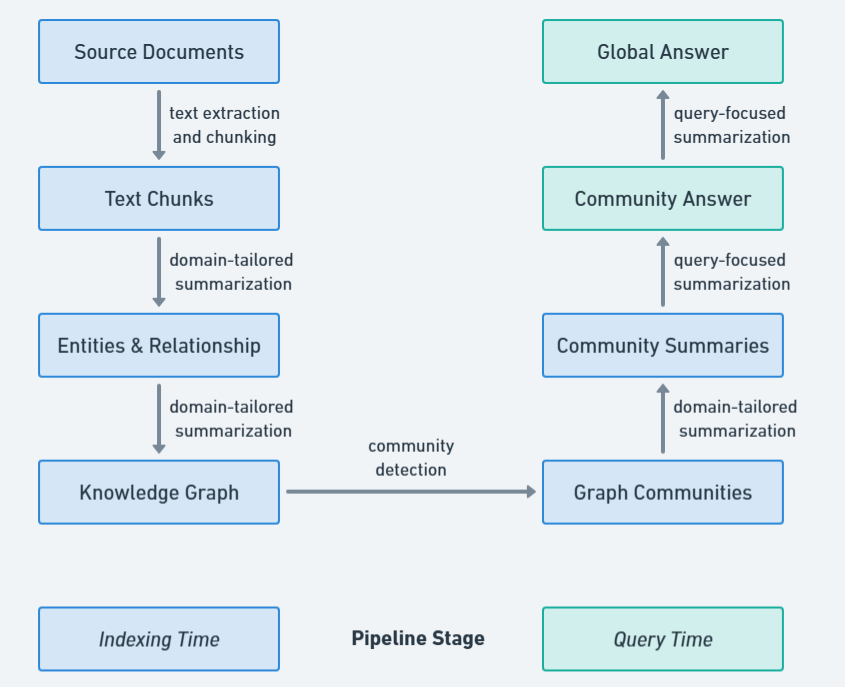
\includegraphics[width=0.6\textwidth]{images/graph-rag-pipeline.png}
	\caption{
		Alur kerja GraphRAG yang memanfaatkan indeks graf dan deteksi komunitas \cite{Edge2025LocalGlobalGraphRAG}
	}
	\label{fig:graphragpipeline}
\end{figure}

Penggunaan graf untuk memodelkan pengetahuan pada arsitektur RAG memberikan beberapa keuntungan dibandingkan RAG berbasis vektor.
Pada RAG konvensional berbasis vektor, sistem akan mengambil sekumpulan dokumen yang secara individu relevan dengan kueri \cite{Lewis2021RAGKnowledgeIntensiveNLP}.
Namun, saat kueri membutuhkan pemahaman \textit{dataset} secara global, RAG konvensional mengalami kesulitan karena basis pengetahuan disusun hanya sebagai potongan dokumen yang saling independen.
Dalam penelitian Edge et al. 2025 yang berjudul "\textit{From Local to Global: A GraphRAG Approach to Query-Focused Summarization}" mengintegrasikan model pengetahuan berbasis \textit{graph} dalam RAG \cite{Edge2025LocalGlobalGraphRAG}.
Alur kerja GraphRAG seperti pada \ref{fig:graphragpipeline} terdiri dari beberapa proses meliputi
\begin{enumerate}
	\item \textbf{\textit{Source Documents \textrightarrow{} Text Chunks}} \\
	      Pada proses ini, dokumen-dokumen awal dipecah menjadi potongan-potongan teks (\textit{text chunks}) dengan ukuran tertentu.
	      Menentukan ukuran dari potongan teks ini merupakan perkara krusial mengingat potongan teks yang panjang mengurangi jumlah kueri ke LLM (hemat biaya) tetapi dapat menurunkan kualitas pengambilan informasi di awal potongan \cite{Edge2025LocalGlobalGraphRAG}.

	\item \textbf{\textit{Text Chunks \textrightarrow{} Entities \& Relationships}} \\
	      LLM akan digunakan sebagai ekstraktor entitas penting, relasi antar entitas, dan deskripsi singkat untuk keduanya dari potongan teks sebelumnya.
	      Klaim yang berupa pernyataan faktual tentang entitas juga akan diekstrak oleh LLM \cite{Edge2025LocalGlobalGraphRAG}.
	      \textit{Prompt} LLM disesuaikan menggunakan teknik \textit{few-shot} yang memberikan beberapa contoh spesifik hasil yang diharapkan agar respons yang diberikan LLM sesuai \cite{LLMisFewShot2020}.

	\item \textbf{\textit{Entities Relationships \textrightarrow{} Knowledge Graph}} \\
	      Entitas, relasi, dan klaim yang telah diekstrak kemudian ditransformasi menjadi \textit{nodes} (entitas) dan \textit{edges} (relasi) dalam sebuah \textit{kowledge graph}.
	      Deskripsi entitas diagregasikan dengan entitas yang berupa \textit{node}.
	      Entitas, relasi, atau klaim dapat terdeteksi lebih dari satu kali karena proses ekstraksi dilakukan secara berulang dari banyak dokumen yang berbeda.
	      Banyaknya duplikasi relasi menjadi bobot dari \textit{edges} \cite{Edge2025LocalGlobalGraphRAG}.

	\item \textbf{\textit{Knowledge Graph \textrightarrow{} Graph Communities}} \\
	      Berdasarkan \textit{graph} yang telah terbentuk sebelumnya, komunitas akan dideteksi menggunaka algoritma tertentu yang bertujuan untuk memartisi \textit{graph} menjadi beberapa komunitas yang terdiri dari kumpulan \textit{nodes} yang terhubung dengan erat.
	      Dalam penelitian ini digunakan \textit{Leiden community detection} (Trag et al. 2019) secara hierarkis, mendeteksi sub-komunitas secara rekursif dalam setiap komunitas yang terdeteksi hingga mencapai komunitas yang tidak dapat lagi dipartisi \cite{Traag2019Leiden}.

	\item \textbf{\textit{Graph Communities \textrightarrow{} Community Summaries}} \\
	      Proses ini membuat ringkasan dari setiap komunitas dalam hierarki komunitas menggunakan metode tertentu.
	      Ringkasan ini secara independen berguna untuk memahami struktur global dan semantik \textit{dataset} serta dapat digunakan untuk memindai korpus tanpa adanya kueri tertentu.
	      Ringkasan berfungsi sebagai bagian dari indeks graf yang digunakan untuk menjawab kueri global \cite{Edge2025LocalGlobalGraphRAG}.

	\item \textbf{\textit{Community Summaries \textrightarrow{} Community Answers \textrightarrow{} Global Answer}} \\
	      Berdasarkan pertanyaan pengguna, ringkasan komunitas yang telah dibuat sebelumnya dapat digunakan untuk menghasilkan jawaban final melalui proses yang bertahap.
	      Ringkasan komunitas diacak dan dibagi menjadi potongan-potongan (\textit{chunks}) dengan ukuran token tertentu.
	      LLM menghasilkan jawaban sementara (\textit{intermediate answers}) dari \textit{chunks} ini secara paralel, beserta skor seberapa membantu jawaban tersebut (0-100).
	      Jawaban dengan skor 0 akan dibuang.
	      Jawaban sementara diurutkan berdasarkan skornya, lalu dimasukkan ke konteks baru LLM hingga batas token tercapai untuk menghasilkan jawaban global (\textit{global answer}) kepada pengguna \cite{Edge2025LocalGlobalGraphRAG}.
\end{enumerate}






\section{Dasar Teori}
\subsection{Kesehatan Mental}
Kesehatan mental, menurut definisi dari \textit{World Health Organization} (WHO), adalah sebuah kondisi kesejahteraan mental (\textit{state of mental well-being})
di mana setiap individu sadar akan potensi yang dimiliki, belajar dan bekerja dengan baik, dan memberikan kontribusi bagi komunitasnya \cite{WHO2022MentalHealth}.
Definisi tersebut menekankan bahwa kesehatan mental bukanlah sekadar kondisi bebas dari gangguan jiwa, melainkan sebuah fondasi yang memungkinkan seseorang untuk berpikir, belajar, merasakan emosi, berinteraksi dengan orang lain, dan menikmati hidup.
Kesehatan mental merupakan komponen yang tidak terpisahkan dengan kesehatan secara keseluruhan dan sama pentingnya dengan kesehatan fisik.

\subsection{\textit{Natural Language Processing}}
Pemrosesan bahasa alami (\textit{Natural Language Processing}, NLP) merupakan serangkaian teknik komputasi yang didorong secara teoritis untuk menganalisis dan merepresentasikan
teks alami pada beberapa tingkat analisis linguistik dengan tujuan mencapai pemrosesan bahasa seperti manusia untuk serangkaian tugas atau aplikasi \cite{Liddy2001NLP}.
Komputer tidak dapat mengerti bahasa manusia yang kompleks dan tidak pasti secara langsung, tetapi memerlukan sesuatu untuk menjadi penghubung antara keduanya.
NLP hadir sebagai cabang dari kecerdasan buatan (AI) yang berfungsi sebagai jembatan antara bahasa manusia yang kompleks dengan komputasi komputer yang terstruktur.
Tujuan utama dari NLP adalah memberdayakan komputer untuk memahami, menafsirkan, memanipulasi, dan menghasilkan bahasa manusia yang bermakna dan bermanfaat.

NLP dapat diklasifikasikan menjadi dua bagian, yaitu \textit{Natural Language Understanding} (NLU) dan \textit{Natural Language Generation} (NLG) \cite{Khurana2022AboutNLP}.
Berikut merupakan penjelasan dari NLU dan NLG.

\begin{enumerate}
	\item \textbf{\textit{Natural Language Understanding} (NLU)} \\
	      NLU memungkinkan komputer untuk memahami bahasa alami dan menganalisisnya dengan mengekstrak konsep, entitas, emosi, kata kunci, dll.
	      NLU berkaitan dengan ilmu bahasa (linguistik) yang berupa morfologi atau bentuk kata, leksikal atau makna kata, sintaksis atau susunan kalimat, semantik atau makna kalimat, \textit{discourse} atau hubungan antar kalimat, dan pragmatik atau makna kontekstual \cite{Khurana2022AboutNLP}.
	\item \textbf{\textit{Natural Language Generation} (NLG)} \\
	      NLG merupakan proses menghasilkan teks, dapat berupa kata, frasa, atau kalimat, yang bermakna dari representasi internal.
	      Proses ini terjadi dalam empat fase yaitu mengidentifikasi tujuan, merencanakan cara mencapai tujuan, mengevaluasi situasi dan sumber komunikasi yang tersedia, dan mewujudkan rencana sebagai teks \cite{Khurana2022AboutNLP}.
\end{enumerate}

Aplikasi NLP sangat luas dan meresap dalam kehidupan sehari-hari, mulai dari fungsionalitas mesin pencari, \textit{chatbot} layanan pelanggan, asisten digital seperti Bixby, Siri dan Alexa, hingga aplikasi khusus seperti analisis sentimen, mesin penerjemah otomatis, dan ekstraksi informasi dari dokumen.
Pada domain kesehatan mental, NLP telah menunjukkan potensi signifikan dalam menganalisis catatan klinis elektronik, unggahan di media sosial, dan respons survei untuk membantu dalam deteksi dini dan pemantauan kondisi seperti depresi, kecemasan, dan \textit{Post-Traumatic Stress Disorder} (PTSD) \cite{NLPonMentalHealth}.

\subsection{\textit{Machine Learning}}
Pembelajaran mesin (\textit{Machine Learning}, ML) adalah bidang AI yang fokus pada pembelajaran dengan mengembangkan algoritma terbaik untuk merepresentasikan data yang tersedia.
Berbeda dengan pemrograman klasik, di mana algoritma dapat dikodekan secara eksplisit menggunakan fitur yang diketahui,
ML menggunakan subset data untuk menghasilkan algoritma yang paling cocok untuk pola data tersebut \cite{choi2020IntroductionML_NN_DL}.
Inti dari ML adalah kemampuannya untuk secara otomatis menemukan pola dalam data dan menggunakan pola tersebut untuk membuat inferensi atau prediksi pada data baru yang belum pernah dilihat.

Algoritma ML membangun model matematis berdasarkan kumpulan data sampel, yang dikenal sebagai "data pelatihan" (\textit{training} data), untuk melakukan berbagai tugas seperti klasifikasi, regresi, atau pengelompokan.
Dalam ML terdapat beberapa metode pembelajaran yang umum digunakan, yaitu \textit{supervised} di mana model belajar dari data yang telah diberi label dengan output yang benar, \textit{unsupervised} di mana model belajar menemukan pola tersembunyi dari data tanpa label, dan \textit{reinforcement} di mana model belajar untuk membuat urutan keputusan dengan berinteraksi dengan lingkungannya untuk memaksimalkan imbalan kumulatif \cite{choi2020IntroductionML_NN_DL}.
Penerapan ML sangat luas, mencakup berbagai domain seperti penyaringan email spam, sistem rekomendasi, pengenalan objek, pengenalan ucapan, diagnosis medis berdasarkan data pasien, dan analisis pasar keuangan untuk prediksi tren.
ML menjadi sangat berguna dalam situasi di mana perancangan dan pengkodean algoritma konvensional yang eksplisit untuk melakukan tugas tertentu dianggap sulit atau tidak praktis karena kompleksitas masalah atau sifat data yang dinamis.


\subsection{\textit{Deep Learning}}
Pembelajaran mendalam (\textit{Deep Learning, DL}) merupakan sebuah pendekatan dalam \textit{Machine learning} yang berusaha mempelajari representasi data melalui struktur model yang terdiri dari banyak lapisan (\textit{layers}) \cite{IanGoodfellow2016DeepLearning}.
Beberapa algoritma pembelajaran yang dikembangkan, awalnya dikembangkan sebagai model komputasi dari pembelajaran biologis yang meniru cara otak bekerja.
Maka dari itu, nama lain dari \textit{deep learning} adalah jaringan saraf tiruan (\textit{Artificial Neural Network}, ANN) \cite{IanGoodfellow2016DeepLearning}.
Jaringan tersebut digunakan untuk mempelajari representasi data dengan berbagai tingkat abstraksi.
Istilah mendalam (\textit{deep}) merujuk pada kedalaman atau banyaknya lapisan dalam jaringan saraf ini.
Setiap lapisan dalam arsitektur DL menerima output dari lapisan sebelumnya, mentransformasikannya, dan meneruskannya ke lapisan berikutnya, secara bertahap mengekstraksi fitur-fitur yang semakin kompleks dan relevan dari data input mentah \cite{IanGoodfellow2016DeepLearning}.

Sebagai subset dari \textit{Machine Learning} (ML), yang juga merupakan subset dari AI, DL memiliki perbedaan signifikan dibandingkan dengan ML.
DL memiliki kemampuan \textit{feature engineering} secara otomatis.
ML konvensional sering kali memerlukan intervensi manusia untuk merancang dan memilih fitur-fitur input yang relevan dari data, model DL dapat secara mandiri mempelajari hierarki fitur yang optimal langsung dari data mentah, seperti piksel dalam gambar atau kata-kata dalam teks \cite{IanGoodfellow2016DeepLearning}.
Aplikasi DL telah merambah berbagai bidang, termasuk pengenalan gambar dan ucapan, deteksi objek dalam video, pemrosesan bahasa alami untuk terjemahan dan pemahaman, serta pengembangan kendaraan otonom.


\subsection{\textit{Large Language Model}}
Model bahasa besar (\textit{Large Language Model}, LLM) merupakan model bahasa berskala besar yang mampu memahami, memprediksi, dan menghasilkan bahasa manusia secara alami dan kontekstual \cite{Chang2024SurveyonLLM}.
LLM merupakan bentuk lanjutan dari \textit{language models} (LMs), yang secara umum adalah sistem komputasi yang mempelajari probabilitas urutan kata dalam teks.
Model bahasa awal seperti \textit{n-gram models} memprediksi kata berikutnya berdasarkan konteks kata-kata sebelumnya, namun memiliki keterbatasan seperti ketidakmampuan menangani kata yang jarang muncul, kecenderungan \textit{overfitting}, serta kesulitan dalam memahami struktur linguistik yang kompleks.
LLM hadir untuk mengatasi tantangan tersebut dengan memanfaatkan arsitektur modern dan kapasitas pembelajaran yang jauh lebih besar \cite{Chang2024SurveyonLLM}.

Keunggulan lain dari LLM terletak pada kemampuan \textit{in-context learning}, yaitu kemampuan untuk melakukan adaptasi dan menyelesaikan berbagai tugas hanya dari petunjuk yang diberikan dalam bentuk \textit{prompt}, tanpa perlu pelatihan ulang secara eksplisit.
LLM dapat "belajar" dari konteks input yang diberikan pengguna untuk memberikan respons yang relevan dan akurat.
Fitur ini membuat LLM sangat fleksibel dan dapat digunakan untuk berbagai keperluan, mulai dari menjawab pertanyaan, membuat ringkasan, menerjemahkan teks, menulis kode program, hingga mengekstrak entitas dari sebuah dokumen \cite{Chang2024SurveyonLLM}.

\subsection{Gemini}
Gemini adalah famili model AI multimoda yang dikembangkan oleh Google DeepMind.
Model Gemini dibangun berdasarkan arsitektur transformer \textit{decoders}.
Model ini dilatih dengan data multimoda dan multilingual yang berasal dari \textit{website}, buku, dan kode, termasuk juga gambar, audio, dan video \cite{saeidnia2023welcomeGemini}.
Saat penelitian dilakukan, Gemini telah berada pada versi 2.5 yang menggunakan arsitektur  \textit{sparse mixture-of-experts} (MoE) \textit{transformer}.
Gemini 2.5 mendukung input konteks dengan panjang lebih dari 1 juta token yang memungkinkan untuk memahami data dengan cakupan yang luas \cite{comanici2025gemini2.5}.



\subsection{GPT}
\textit{Generative Pre-trained Transformer} (GPT) adalah \textit{language model} berbasis arsitektur transformer yang dikembangkan oleh OpenAI sejak tahun 2018 saat rilis model transformer pertamanya.
Saat penelitian ini dilakukan, OpenAI telah memperbarui model GPT hingga generasi keempat seperti gpt-4.1.
Model ini dilatih secara unsupervised pada kumpulan data dalam jumlah besar yang berasal dari \textit{website} publik, kode dan data matematis, serta data multimodal seperti gambar, audio, dan video.
Pelatihan tersebut bertujuan untuk memahami pola bahasa alami, lalu digunakan untuk menghasilkan teks baru yang koheren.
GPT bekerja dengan mekanisme \textit{self-attention} yang memungkinkan model memahami konteks panjang dalam sebuah teks, sehingga mampu menghasilkan jawaban yang relevan dan konsisten \cite{hurst2024gpt4o}.

\subsection{\textit{Retrieval-Augmented Generation}}
\textit{Retrieval-Augmented Generation} (RAG) adalah teknik yang menggabungkan kekuatan \textit{Large Language Model} (LLM) dengan sistem pengambilan (\textit{retrieval}) informasi dari sumber eksternal (seperti basis pengetahuan atau dokumen) untuk meningkatkan akurasi, ketepatan, dan kedalaman pengetahuan dalam tugas \textit{knowledge-intensive} seperti tanya-jawab terbuka atau penjelasan faktual.
Tujuan utama RAG adalah untuk mengatasi beberapa keterbatasan yang melekat pada LLM standar, seperti kecenderungan untuk menghasilkan informasi yang tidak akurat atau "berhalusinasi", menyajikan pengetahuan yang tidak relevan, atau kurangnya kemampuan untuk menyediakan sumber atau justifikasi atas informasi yang dihasilkannya \cite{Lewis2021RAGKnowledgeIntensiveNLP}.


\subsection{Token}
Dalam bidang \textit{Natural Language Processing} (NLP), token merujuk pada satuan terkecil dari teks yang dapat dikenali dan diproses oleh sistem komputasi bahasa.
Token dapat berupa kata, bagian dari kata (\textit{subword}), tanda baca, atau bahkan karakter individual, tergantung pada strategi tokenisasi yang digunakan \cite{Jurafsky2023SpeechLangageProcessing}.
Proses pemecahan teks menjadi token disebut tokenisasi, dan merupakan tahap awal penting dalam \textit{pipeline} pemrosesan bahasa alami.
Dalam model \textit{Large Language Model} seperti GPT atau BERT, tokenisasi umumnya dilakukan dengan pendekatan berbasis \textit{subword}, seperti \textit{Byte Pair Encoding} (BPE) atau WordPiece, yang memungkinkan model mengenali dan memproses kata-kata baru atau langka dengan efisien \cite{bostrom2020BytePairWordPieceToken}.
Tokenisasi berbasis \textit{subword} menyusun token dari unit-unit kata yang lebih kecil sehingga kosakata tetap terbatas namun tetap mencakup variasi linguistik yang luas.
Misalnya, kata "memperjuangkan" dapat dipecah menjadi beberapa token seperti "mem", "perjuang", dan "kan".


\subsection{Vektor}
Vektor adalah sebuah objek matematis yang memiliki dua karakteristik utama yaitu magnitudo (besar) dan arah.
Secara fundamental, sebuah vektor dapat direpresentasikan sebagai sebuah larik (\textit{array}) terurut yang berisi angka.
Vektor tersebut merupakan elemen dari suatu ruang vektor (\textit{vector space}) yang merupakan himpunan objek yang memiliki operasi penjumlahan dan perkalian skalar serta memenuhi sejumlah aksioma tertentu \cite{strang2009IntroductionLinearAlgebra}.
Sebuah vektor dalam ruang berdimensi $n$ dapat direpresentasikan sebagai barisan terurut dari $n$ bilangan real seperti pada Persamaan \ref{eq:vector}.
\def\V{
	\begin{bmatrix}
		v_1    \\
		v_2    \\
		\vdots \\
		v_n
	\end{bmatrix}
}

\begin{equation}
	\mathbf{v} = \V \in \mathbb{R}^n
	\label{eq:vector}
\end{equation}%
dengan $v_1, v_2, \cdots, v_n$ adalah komponen-komponen dari vektor $\mathbf{v}$ dan $n$ adalah dimensi ruang tempat vektor tersebut berada.
Dalam konteks kecerdasan buatan, vektor biasanya digunakan untuk merepresentasikan objek kompleks seperti teks, gambar, atau video ke dalam bentuk numerik yang dapat diproses oleh mesin.


\subsection{\textit{Cosine Similarity}}
Kesamaan kosinus (\textit{cosine similarity}) merupakan salah satu metrik matematis untuk yang digunakan untuk mengukur tingkat kemiripan antara dua vektor \textit{non-zero}.
Secara fundamental, metrik ini menghitung nilai kosinus dari sudut yang dibentuk oleh dua vektor tersebut.
Fokus utama dari \textit{cosine similarity} adalah pada orientasi atau arah vektor-vektor tersebut dan mengabaikan besar atau magnitudonya \cite{Xia2015CosineSimilarity}.
Hal ini menjadikannya sangat berguna dalam konteks di mana besaran absolut dari vektor kurang relevan dibandingkan dengan "arah" atau "profil" relatifnya.
Secara matematis, formula untuk menghitung nilai \textit{cosine similarity} dapat diungkapkan dengan Persamaan \ref{eq:cosine-similarity}.

\begin{equation}
	\text{$Similarity$}(\vec{A}, \vec{B}) = \cos{(\theta)} = \frac{\vec{A} \cdot \vec{B}}{\|\vec{A}\| \|\vec{B}\|} = \frac{\sum_{i=1}^{n} A_i B_i}{\sqrt{\sum_{i=1}^{n} A_i^2} \sqrt{\sum_{i=1}^{n} B_i^2}}
	\label{eq:cosine-similarity}
\end{equation}%
dengan $\vec{A} \cdot \vec{B}$ adalah \textit{dot product} dari vektor $A$ dan $B$, $\|\vec{A}\|$ adalah magnitudo atau besar dari vektor $A$ dan $\|\vec{B}\|$ adalah magnitudo atau besar dari vektor $B$.
\textit{Dot product} $\vec{A} \cdot \vec{B}$ dilakukan dengan mengalikan komponen-komponen yang bersesuaian dari kedua vektor kemudian menjumlahkan hasilnya.
Magnitudo dari sebuah vektor dihitung sebagai akar kuadrat dari jumlah kuadrat setiap komponennya.
Nilai \textit{cosine similarity} akan selalu berada pada rentang $-1$ hingga $1$.
Nilai $1$ menunjukkan bahwa kedua vektor memiliki orientasi yang sama persis atau sudut yang dibentuk keduanya 0 derajat.
Nilai $0$ menunjukkan bahwa kedua vektor ortogonal atau saling tegak lurus (sudut 90 derajat) yang sering diartikan sebagai tidak adanya kesamaan orientasi.
Nilai $-1$ menunjukkan bahwa kedua vektor memiliki orientasi yang berlawanan arah (sudut 180 derajat).
Dua buah vektor dikatakan mirip apabila nilai \textit{cosine similarity} antar keduanya mendekati $1$.


\subsection{\textit{Vector Embedding}}
\textit{Vector embedding} merupakan representasi numerik dari sebuah data, terutama yang tidak terstruktur seperti teks, gambar, audio, atau video.
Pada prinsipnya \textit{vector embedding} bekerja dengan melakukan transformasi data ke dalam bentuk vektor berdimensi tinggi.
Bentuk vektor tersebut merepresentasikan fitur atau karakteristik dari objek asli, seperti makna dalam teks, objek dalam gambar, atau suara dalam audio.
Dalam konteks NLP \textit{embedding} digunakan untuk menangkap hubungan semantik, sintaksis, atau kontekstual yang mendasari sebuah teks.
Hal tersebut membuat hubungan antar objek seperti kemiripan semantik teks dapat dianalisis secara matematis \cite{Singh2023EmbeddingVectorAndVectorDB}.

Proses pembentukan \textit{vector embedding} biasanya melibatkan model \textit{machine learning} tradisional seperti Word2Vec dan GloVe atau model berbasis \textit{transformer} yang lebih modern seperti BERT, GPT, dan Gemini.
Model-model tersebut telah dilatih untuk menghasilkan nilai-nilai dalam \textit{vector embedding} berdasarkan makna atau konteks setiap unit data.
Model tradisional seperti GloVe bekerja dengan mentransformasi setiap kata menjadi 1 representasi vektor unik tanpa memperhatikan bagai mana kata tersebut digunakan dalam kalimat.
Sebaliknya, model yang lebih modern seperti BERT, GPT, dan Gemini mampu menghasilkan representasi vektor yang berbeda untuk kata yang sama tergantung pada konteks spesifik kalimat di mana kata tersebut muncul.

\subsection{\textit{Full-Text Search}}
Dalam konteks \textit{information retrieval}, \textit{full-text search} merujuk kepada teknik untuk melakukan pencarian keseluruhan konten tekstual dari sebuah atau koleksi dokumen yang tersimpan.
\textit{Full-text search} adalah jenis pencarian yang dilakukan dengan mencocokkan istilah (\textit{terms}) yang terkandung dalam kueri pencarian dengan \textit{terms} dalam setiap dokumen dalam basis data, kemudian hasilnya di-\textit{ranking} dengan algoritma tertentu.
Jenis pencarian ini banyak digunakan di berbagai bidang, mencakup pencarian bahasa alami yang banyak dijumpai pada mesin pencari, pencarian situs web, dan banyak basis data \cite{beall2008weaknesses}.
Keunggulan utama dari metode pencarian ini adalah kemampuannya dalam menangani variasi teks, termasuk \textit{stemming}, \textit{stopwords}, dan peringkat relevansi hasil.
Misalnya, sistem dapat mendeteksi bahwa kata “berlari” dan “lari” memiliki makna dasar yang sama, sehingga hasil pencarian menjadi lebih akurat.
Dalam implementasi modern, \textit{full-text search} biasanya dilengkapi dengan teknik seperti \textit{inverted index}, \textit{ranking model}, dan skor relevansi \cite{mongodb2025fulltext}.

\subsection{\textit{Vector Database}}
Basis data vektor (\textit{vector database}) adalah salah satu jenis basis data yang dirancang khusus untuk secara efektif mengelola data yang direpresentasikan sebagai vektor berdimensi tinggi.
Vektor-vektor tersebut merupakan representasi numeris dari fitur atau atribut suatu objek yang umumnya dibentuk melalui proses \textit{vector embedding}.
Setiap vektor dapat memiliki puluhan hingga ribuan dimensi tergantung pada kompleksitas data yang direpresentasikan.
Vektor-vektor ini kemudian sering kali dikelompokkan atau diindeks berdasarkan kedekatan mereka dalam ruang vektor multidimensi untuk memudahkan dalam pencarian \cite{Han2023VectorDB_ANN_SimilaritySearch}.

Basis vektor berbeda secara fundamental dengan basis data relasional berbasis baris dan kolom, basis data ini unggul dalam menangani volume besar data tidak terstruktur yang telah ditransformasikan menjadi representasi vektor padat berdimensi tinggi.
Fitur kueri pencarian kemiripan (\textit{similarity search}) menjadikannya sangat unggul dibandingkan basis data lain karena fitur tersebut merupakan operasi krusial bagi banyak aplikasi AI.
Umumnya basis data vektor seperti ChromaDB, Pinecone, Melvis, dll. mendukung algoritma \textit{Approximate Nearest Neighbor} (ANN) yang efisien untuk menemukan vektor-vektor yang paling mirip dengan vektor kueri dalam data yang sangat besar \cite{Han2023VectorDB_ANN_SimilaritySearch}.
Hal tersebut menjadikannya pilihan utama saat berinteraksi dengan data berbentuk vektor.

\subsection{\textit{Graph Database}}
Basis data graf (\textit{graph database}) adalah basis data yang dirancang untuk secara efisien mengelola data yang dimodelkan dalam bentuk graf.
Struktur data pada basis data graf secara fundamental terdiri atas \textit{node} atau \textit{vertex} yang merepresentasikan sebuah entitas atau objek dan \textit{edge} yang merepresentasikan koneksi atau relasi antar node tersebut.
Baik \textit{node}, maupun \textit{edge} dapat memiliki properti yang menyimpan atribut atau metadata yang dapat berisi deskripsi dari entitas atau relasi tersebut \cite{Paul2019GraphDB}.
Salah satu keunggulan dari basis data graf adalah adanya konsep \textit{index-free adjacency} yang berarti setiap \textit{node} dapat secara langsung mengetahui dan dapat mengakses \textit{node} lain yang berhubungan tanpa harus menggunakan indeks tambahan seperti pada basis data relasional.
Hal tersebut mempercepat performa pencarian hubungan antar \textit{node} dan memungkinkan algoritma seperti \textit{graph traversal} yang efisien \cite{Paul2019GraphDB}.

\subsection{\textit{Knowledge Graph}}
Konsep Graf Pengetahuan (\textit{Knowledge Graph}, KG) pertama kali diperkenalkan secara luas oleh Google pada tahun 2012 melalui proyek Google \textit{Knowledge Graph} untuk meningkatkan relevansi hasil pencarian dan pengalaman pencarian pengguna \cite{Singhal2012IntroducingKnowledgeGraph}.
Bermula dari itu, banyak perusahaan dan institusi mengembangkan KG mereka sendiri seperti Bing dengan Stori, DBpedia, YAGO, Wikidata, dan Freebase sebagai bagian dari \textit{semantic web} \cite{Paulheim2016KnowledgeGraphSurvei}.
\textit{Knowledge Graph} adalah representasi semantik terstruktur dari pengetahuan yang memodelkan entitas (seperti orang, tempat, organisasi, dll.) dan hubungan antar entitas dalam bentuk graf.
Setiap entitas direpresentasikan sebagai \textit{node} dan relasi antar entitas direpresentasikan sebagai \textit{edge} \cite{Chen2020ReviewKnowldgeReasoningOverKnowledgeGraph}.
Secara matematis, sebuah struktur KG dapat direpresentasikan dengan Persamaan \ref{eq:knowledge-graph}
\begin{equation}
	\text{$KG$} = \langle E, R, T \rangle
	\label{eq:knowledge-graph}
\end{equation}%
dengan $E$ adalah himpunan semua \textit{node} atau entitas dalam pengetahuan, $R$ adalah himpunan semua relasi, dan $T$ adalah himpunan triplet yang merepresentasikan fakta.
$T$ dapat dinyatakan secara matematis, seperti pada Persamaan \ref{eq:triple-in-kg}

\begin{equation}
	T = \{(h,r,t) \mid h,t \in E, r \in R\}
	\label{eq:triple-in-kg}
\end{equation}

Setiap triplet $T$ terdiri dari tiga bagian yaitu $h$ (\textit{head}) adalah entitas asal, $r$ adalah relasi, dan $t$ (\textit{tail}) adalah entitas tujuan.

\subsection{\textit{Knowledge Extraction}}
Ekstraksi pengetahuan (\textit{Knowledge Extraction}, KE) merupakan proses sistematis untuk mengidentifikasi dan mengekstrak informasi bermakna dari data tidak terstruktur atau semi terstruktur seperti teks untuk direpresentasikan ke dalam bentuk terstruktur yang dapat dipahami oleh mesin.
Dalam konteks \textit{Knowledge Graph}, sumber data yang berupa dokumen akan diekstrak menjadi bentuk triplet (subjek-predikat-objek) yang akan membentuk KG.
Pada praktiknya proses ekstraksi ini terdiri dari ekstraksi entitas, relasi antar entitas, dan klasifikasi entitas.
Proses ini merupakan tahap awal yang krusial dalam konstruksi KG karena akan menentukan kualitas representasi pengetahuan oleh \textit{Knowledge Graph} \cite{Choi2025KnowledgeGraphConstruction}.

\subsection{\textit{Knowledge Retrieval}}
Pengambilan pengetahuan (\textit{Knowledge Retrieval}, KR) merupakan proses pencarian dan pengambilan pengetahuan secara sistematis dari basis data pengetahuan seperti \textit{Knowledge Graph} \cite{Yao2007KnowledgeRetrieval}.
Dalam konteks KG, proses pengambilan ini memungkinkan suatu sistem untuk melakukan inferensi logis dan menjawab kueri secara presisi dan benar.
Penekanan utama dalam \textit{Knowledge Retrieval} adalah pada pengambilan pengetahuan yaitu representasi formal pengetahuan yang dapat diolah untuk penalaran, bukan sekadar pengambilan data mentah atau informasi yang terkait dengan kueri.
KR bertujuan untuk mengambil makna dan hubungan terstruktur yang kemudian dapat dimanfaatkan untuk tugas lain yang lebih kompleks.

\subsection{\textit{Precision}}
\textit{Precision} (presisi) merupakan metrik yang mengukur seberapa banyak item yang berhasil diidentifikasi (\textit{retrieved}) yang benar-benar relevan.
Metrik ini juga dikenal sebagai \textit{confidence} dalam bidang \textit{data mining} dan menjadi fokus utama dalam \textit{information retrieval} dan \textit{machine learning} untuk mengukur keyakinan pada hasil prediksi.
Presisi menunjukkan proporsi kasus positif yang diprediksi dengan positif yang sebenarnya \cite{powers2020evaluationprecisionrecallfmeasure}.
Definisi \textit{Precision} diberikan pada Persamaan \ref{eq:precision}.

\begin{equation}
	\label{eq:precision}
	Precision = \frac{TP}{TP + FP}
	= \frac{\textit{Relevant items retrieved}}{\textit{Retrieved items}}
\end{equation}%
dengan:
\begin{itemize}
	\item $TP$ adalah \textit{True Positives}, yaitu jumlah prediksi positif yang benar.
	\item $FP$ adalah \textit{False Positives}, yaitu jumlah prediksi positif yang salah.
\end{itemize}

Dalam kasus RAG, presisi berarti proporsi banyaknya informasi relevan dari semua informasi yang dihasilkan dibandingkan dengan total informasi yang dihasilkan.
Metrik ini dapat menunjukkan tingkat \textit{noise} dari konteks yang dihasilkan \textit{retriever}.

\subsection{\textit{Recall}}

\textit{Recall} merupakan metrik yang mengukur seberapa banyak item relevan yang berhasil diidentifikasi dari semua item yang relevan.
Metrik ini juga dikenal sebagai \textit{sensitivity} atau \textit{True Positive Rate} (TPR).
\textit{Recall} menunjukkan proporsi kasus positif yang diprediksi dengan total kasus positif yang seharusnya muncul \cite{powers2020evaluationprecisionrecallfmeasure}.
Definisi \textit{Recall} diberikan pada Persamaan \ref{eq:recall}.

\begin{equation}
	\label{eq:recall}
	Recall = \frac{TP}{TP + FN} = \frac{\textit{Relevant items retrieved}}{\textit{Relevant items}}
\end{equation}%
dengan:
\begin{itemize}
	\item $TP$ adalah \textit{True Positives}, yaitu jumlah prediksi positif yang benar.
	\item $FN$ adalah \textit{False Negatives}, yaitu jumlah kasus positif yang gagal diprediksi (salah diprediksi negatif).
\end{itemize}

Dalam kasus RAG \textit{recall} berarti proporsi banyaknya informasi relevan dari semua informasi yang dihasilkan dibandingkan dengan total informasi relevan yang seharusnya muncul.
Metrik ini dapat menunjukkan seberapa banyak informasi relevan yang dihasilkan \textit{retriever} dari yang seharusnya muncul.

\subsection{\textit{Mean Reciprocal Rank} (MRR)}
Metrik \textit{Reciprocal Rank} (RR) menghitung kebalikan dari peringkat (\textit{rank}) di mana dokumen relevan pertama ditemukan.
RR bernilai 1 jika dokumen relevan ditemukan pada peringkat 1,  0,5 jika ditemukan pada peringkat 2,  0,33 pada peringkat 3, dan seterusnya.
Ketika dirata-ratakan di seluruh kueri, ukuran ini disebut \textit{Mean Reciprocal Rank} (MRR) \cite{craswell2016meanMRR}.
MRR didefinisikan dalam Persamaan \ref{eq:mrr}

\begin{equation}
	\label{eq:mrr}
	\mathrm{MRR} = \frac{1}{N} \sum_{i=1}^{N} \frac{1}{\text{rank}_i}
\end{equation}

Dalam konteks RAG, MRR menunjukkan performa \textit{retriever} dalam memprioritaskan urutan munculnya konteks yang relevan.
Hal tersebut cukup krusial karena beberapa LLM memiliki kecenderungan memprioritaskan informasi yang muncul di awal.

\subsection{\textit{Retrieval-Augmented Generation Assessment} (RAGAS) \textit{Framework}}

RAGAS (\textit{Retrieval-Augmented Generation Assessment}) adalah sebuah kerangka kerja yang dirancang untuk mengevaluasi sistem AI yang menggunakan arsitektur \textit{Retrieval-Augmented Generation} (RAG).
Tujuan utamanya adalah untuk mengatasi tantangan dalam menilai kualitas \textit{pipeline} RAG, yang terdiri dari komponen pengambilan (\textit{retrieval}) dan generasi (\textit{generation}).
Kerangka kerja ini menyediakan serangkaian metrik otomatis yang dapat mengukur berbagai aspek kinerja berbasis LLM sehingga mampu untuk mengevaluasi data dalam bentuk bahasa alami.
Dengan demikian, RAGAS memungkinkan pengembang untuk secara efisien mendiagnosis kelemahan, baik pada kemampuan sistem untuk menemukan informasi yang relevan, maupun pada kemampuannya untuk menghasilkan jawaban yang akurat dan koheren dari informasi tersebut \cite{es2024ragas}.

Untuk memberikan evaluasi yang komprehensif, RAGAS menyediakan beberapa metrik utama untuk mengevaluasi sistem RAG.

\begin{enumerate}
	\item \textbf{\textit{Faithfulness}} \\
	      Metrik pertama adalah \textit{faithfulness} atau kepatuhan.
	      \textit{Faithfulness} adalah metrik krusial yang mengukur konsistensi faktual jawaban yang dihasilkan terhadap konteks yang diambil.
	      Metrik ini memastikan bahwa model tidak berhalusinasi dengan memverifikasi bahwa setiap klaim dalam jawaban didukung oleh sumber yang diberikan.
	\item \textbf{\textit{Response Relevancy}} \\
	      \textit{Response Relevancy} menilai seberapa relevan jawaban terhadap pertanyaan asli.
	      Jawaban yang tidak lengkap atau mengandung informasi berlebihan yang tidak diminta akan dikenakan penalti.
	      Semakin tinggi nilainya menunjukkan respons selaras dengan pertanyaan, sedangkan semakin kecil nilainya menunjukkan respons kurang lengkap atau mengandung informasi yang redundan.
	      Metrik ini tidak mengukur kebenaran, melainkan fokus pada ketepatan dalam menjawab pertanyaan.
	\item \textbf{\textit{Answer Similarity}} \\
	      \textit{Answer Similarity} secara spesifik mengukur kemiripan semantik antara jawaban yang dihasilkan dan jawaban referensi, biasanya dihitung menggunakan \textit{cosine similarity} dari \textit{embedding} kedua jawaban tersebut.
	      Secara bersama-sama, metrik-metrik ini memberikan pandangan holistik yang memungkinkan pengembang untuk memahami secara mendalam apakah jawaban yang dihasilkan tidak hanya relevan dan setia pada konteks, tetapi juga benar dan mirip secara semantik dengan jawaban yang ideal.
	\item \textbf{\textit{Correctness}} \\
	      Selanjutnya, \textit{Correctness} mengevaluasi keakuratan jawaban secara keseluruhan dengan membandingkannya dengan jawaban referensi (\textit{ground truth}).
	      Metrik ini bergantung pada \textit{ground truth} dan jawaban, dengan skor berkisar antara 0 hingga 1.
	      Skor yang lebih tinggi menunjukkan kesesuaian yang lebih dekat antara jawaban yang dihasilkan dan kebenaran dasar, yang menandakan ketepatan yang lebih baik.
\end{enumerate}


\section{Analisis Perbandingan Metode}

Dalam tinjauan pustaka telah diulas berbagai metode untuk mengembangkan \textit{chatbot}.
Komparasi dari masing-masing metode tersebut terdapat pada Tabel \ref{tab:method-comparision}.

\begin{longtable}{|p{4cm}|p{5cm}|p{5cm}|}
	\caption{Ringkasan dan Perbandingan Metode Pengembangan \textit{Chatbot}} \label{tab:method-comparision} \\
	\hline
	\textbf{Metode} & \textbf{Kelebihan} & \textbf{Kekurangan}                                               \\
	\hline
	\endfirsthead

	\hline
	\textbf{Metode} & \textbf{Kelebihan} & \textbf{Kekurangan}                                               \\
	\hline
	\endhead

	\hline
	\endfoot

	\textbf{\textit{Fine-Tuning LLM}: }
	Melatih lebih lanjut sebuah \textit{Large Language Model} (LLM) yang sudah ada dengan menggunakan \textit{dataset} spesifik domain.
	Tujuannya adalah untuk mengadaptasi pengetahuan dan gaya respons model agar sesuai dengan kebutuhan.
	                &
	\begin{enumerate}
		\item Menghasilkan respons yang sangat relevan dan akurat untuk domain spesifik.
		\item Gaya bahasa dan "kepribadian" \textit{chatbot} dapat disesuaikan.
		\item Latensi lebih rendah saat inferensi karena tidak butuh konteks eksternal.
	\end{enumerate}
	                &
	\begin{enumerate}
		\item Membutuhkan \textit{dataset} pelatihan yang besar dan berkualitas tinggi.
		\item Prosesnya mahal secara komputasi dan memakan waktu.
		\item Pengetahuan sulit diperbarui tanpa melatih ulang.
		\item Masih rentan terhadap "halusinasi".
	\end{enumerate}
	\\
	\hline
	\textbf{\textit{Prompt Engineering LLM}: }
	Merancang dan menyusun instruksi (\textit{prompt}) yang detail dan terstruktur untuk mengarahkan LLM agar memberikan respons yang diinginkan tanpa mengubah model itu sendiri.
	                &
	\begin{enumerate}
		\item Tidak memerlukan pelatihan ulang.
		\item Biaya rendah dan fleksibel.
		\item Sangat mudah dilakukan pembaruan sesuai kebutuhan.
	\end{enumerate}
	                &
	\begin{enumerate}
		\item Performa sangat tergantung kualitas \textit{prompt}.
		\item Konsistensi jawaban tidak selalu terjamin.
		\item Sulit untuk menangani domain yang sangat spesifik.
	\end{enumerate}
	\\
	\hline
	\textbf{\textit{Retrieval-Augmented Generation} Konvensional: }
	Menggabungkan LLM dengan sistem pencarian informasi dari basis data eksternal (misalnya, dokumen teks).
	Sebelum menjawab, sistem mencari informasi relevan terlebih dahulu, lalu memberikannya sebagai konteks bagi LLM.
	                &
	\begin{enumerate}
		\item Mengurangi halusinasi karena jawaban didasarkan pada sumber nyata.
		\item Memudahkan pembaruan informasi tanpa proses \textit{training} ulang.
	\end{enumerate}
	                &
	\begin{enumerate}
		\item Kualitas jawaban sangat bergantung pada kualitas \textit{retriever}.
		\item Butuh \textit{pipeline} tambahan untuk pencarian data yang dapat menambah latensi.
	\end{enumerate}
	\\
	\hline
	\textbf{\textit{Retrieval-Augmented Generation} dengan \textit{Knowledge Graph}: }
	Varian dari RAG yang menggunakan \textit{Knowledge Graph} (KG) sebagai basis data eksternal.
	KG merepresentasikan informasi sebagai entitas dan hubungan yang terstruktur, memberikan konteks yang lebih kaya kepada LLM.
	                &
	\begin{enumerate}
		\item Lebih terstruktur dalam memodelkan informasi dibanding dokumen teks biasa.
		\item Mendukung pencarian dengan konteks yang lebih luas.
		\item Memperkuat konteks relasional antar data.
		\item Dapat meng-\textit{update} informasi tanpa \textit{retraining}.
	\end{enumerate}
	                &
	\begin{enumerate}
		\item Pembuatan \textit{Knowledge Graph} memerlukan pemodelan yang optimal.
		\item Kompleksitas implementasi tinggi.
	\end{enumerate}
	\\
	\hline
\end{longtable}

Metode \textit{Fine-Tuning} LLM menawarkan beberapa keunggulan utama, seperti kemampuan untuk menghasilkan respons yang sangat relevan dan akurat untuk domain spesifik.
Selain itu, metode ini memungkinkan pengembang untuk menyesuaikan gaya bahasa dan "kepribadian" \textit{chatbot}, yang didukung oleh latensi yang lebih rendah karena tidak memerlukan konteks eksternal saat inferensi.

Namun, di balik kelebihannya, terdapat kekurangan yang signifikan, proses \textit{fine-tuning} membutuhkan \textit{dataset} pelatihan yang besar dan berkualitas tinggi, menjadikannya mahal dan memakan waktu secara komputasi.
Pengetahuan yang ditanamkan ke dalam model juga bersifat statis, sehingga sulit untuk diperbarui tanpa melalui proses pelatihan ulang yang intensif.
Kelemahan yang paling krusial adalah metode ini masih rentan terhadap "halusinasi", yaitu memberikan informasi yang salah atau tidak faktual.

Dalam konteks yang sangat sensitif seperti layanan kesehatan mental, risiko halusinasi dari metode \textit{fine-tuning} menjadi opsi yang riskan.
Oleh karena itu, metode RAG berbasis \textit{\textit{Knowledge Graph}} muncul sebagai solusi yang lebih unggul.
Dengan mendasarkan jawaban pada basis data terstruktur yang memetakan entitas dan relasinya, RAG dengan KG secara signifikan mengurangi ambiguitas dan meningkatkan akurasi fakta.
Kemampuannya untuk melakukan penalaran yang kompleks berdasarkan sumber terverifikasi menjadikannya pilihan yang lebih aman dan andal untuk membangun \textit{chatbot} kesehatan mental yang bertanggung jawab.
